\section{Introduction}
\label{sec:introduction}

PID controllers account for more than 90\% of deployed control loops in
industrial process control~\cite{Aastrom2006}, yet selecting appropriate
gains remains a practical challenge.
Classical tuning rules --- Ziegler--Nichols (ZN)~\cite{ZieglerNichols1942},
Cohen--Coon~\cite{CohenCoon1953}, IMC~\cite{Rivera1986} --- require an
open-loop step test or explicit prior knowledge of the process.
In industrial settings such tests are often infeasible due to production
constraints or safety requirements.

Bang-Bang (two-point) controllers are already widely deployed as thermostats
and safety limiters in cooling, heating, and refrigeration plants.
They inherently drive the closed loop into a limit-cycle oscillation that
encodes the plant dynamics.
\Cref{fig:intro_duty_cycle} illustrates this: the duty cycle shifts with
setpoint, reflecting the steady-state gain, while the waveform shape carries
information about the time constant and dead time.

\begin{figure}[htbp][t]
    \centering
    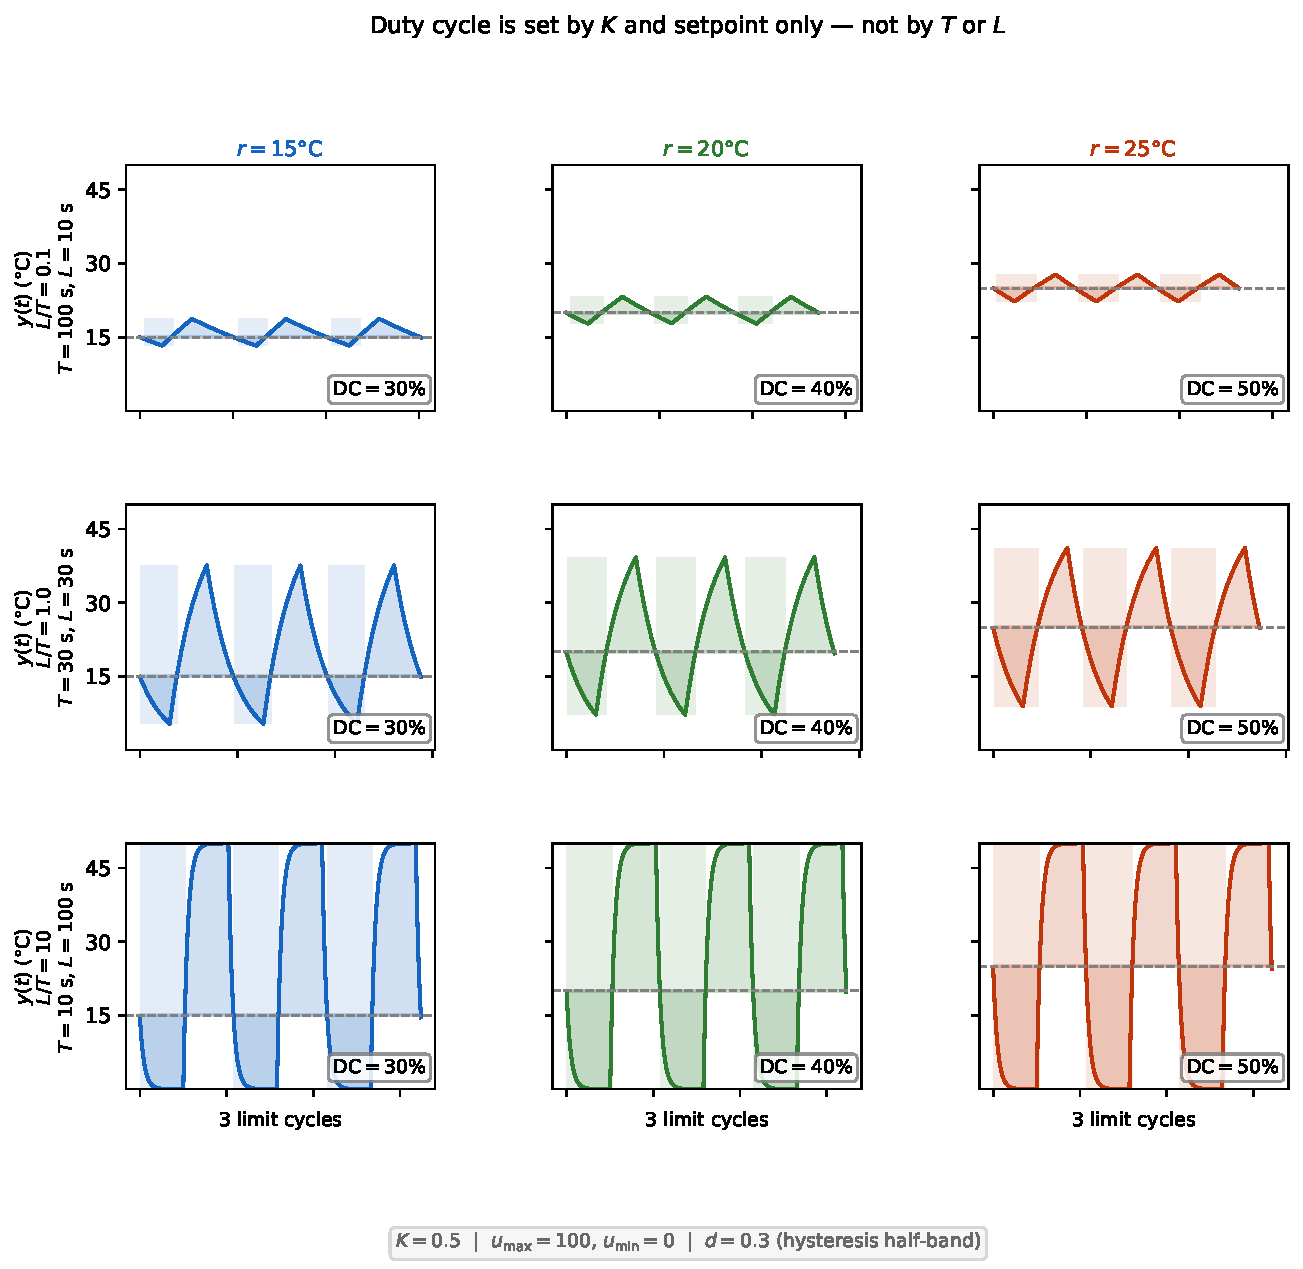
\includegraphics[width=0.96\linewidth]{figures/intro_duty_cycle.pdf}
    \caption{Bang-Bang limit cycles at three setpoints
             ($r \in \{15, 20, 25\}$~\textdegree C)
             for three FOPDT plants sharing the same gain $K$ but different
             $L/T$ ratios:
             lag-dominated ($L/T=0.1$, $T=\SI{100}{\second}$, $L=\SI{10}{\second}$),
             balanced ($L/T=1.0$, $T=\SI{30}{\second}$, $L=\SI{30}{\second}$), and
             dead-time dominant ($L/T=10$, $T=\SI{10}{\second}$, $L=\SI{100}{\second}$).
             Each panel shows the plant output $y(t)$ with the ON-phase
             tinted and the duty cycle (DC) annotated.
             The DC values are identical across all three plants at every setpoint,
             confirming that duty cycle depends only on $K$ and $r$ ---
             not on $T$ or $L$. The oscillation period and waveform shape do
             differ, which is why the KZV extracts $T$ and $L$ separately.}
    \label{fig:intro_duty_cycle}
\end{figure}

\subsection{The KZV Approach}
\label{sec:kzv_intro}

This paper presents the \emph{Kiwitsche 2-Punkt-Verfahren} (KZV): a
four-phase procedure that exploits the Bang-Bang limit cycle to identify the
plant's FOPDT model and synthesise an IMC-PID controller without any
additional open-loop experiment.
The KZV is a specialised variant of the relay-feedback idea of
\AA{}str\"{o}m and H\"{a}gglund~\cite{Astrom1984}: instead of reading a single
Nyquist point, it uses time-domain transient slopes within each half-cycle to
extract the full FOPDT triple $(K,\,T,\,L)$.
\Cref{fig:intro_phase_portrait} shows the phase-plane orbits produced by the
same plant at three setpoints --- each orbit is a reproducible fingerprint of
the local plant dynamics.

\begin{figure}[htbp]
    \centering
    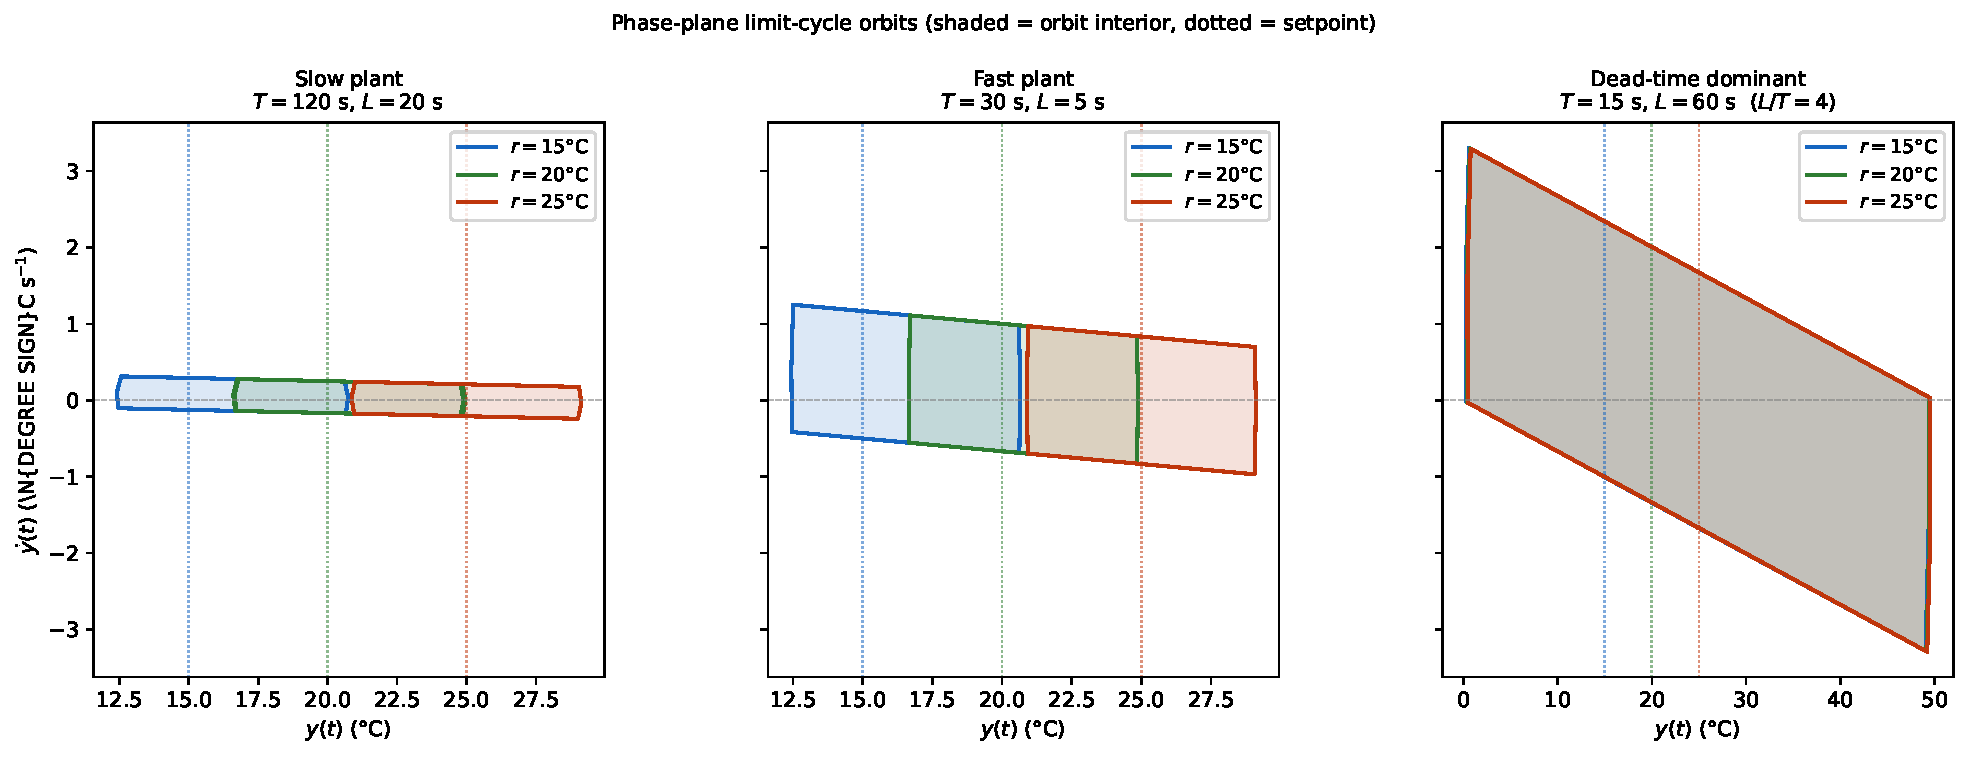
\includegraphics[width=0.96\linewidth]{figures/intro_phase_portrait.pdf}
    \caption{Phase-plane limit-cycle orbits ($y$ vs.\ $\dot{y}$) at
             $r \in \{15, 20, 25\}$~\textdegree C.
             Each closed curve encodes the local FOPDT parameters at that
             operating point.}
    \label{fig:intro_phase_portrait}
\end{figure}

\Cref{sec:theory} reviews the theoretical foundations;
\cref{sec:methodology} details the KZV procedure;
\cref{sec:results} presents simulation results; and
\cref{sec:conclusion} concludes.
